%! Author = madi
%! Date = 25.05.2021

% Preamble
\documentclass{article}
\usepackage{graphicx}



\graphicspath{{./images/} }
\setlength\parindent{0pt}

\hypersetup{
    colorlinks,
    linkcolor={cyan!50!black},
    citecolor={blue!50!black},
    urlcolor={blue!80!black}
}

\makeatletter
\newcommand{\sectionauthor}[1]{
        {\parindent 0em \large \scshape Autor: #1 \par \nobreak \vspace{1em}}
    @afterheading
}
\newcommand{\specification}[3]{
        {\parindent 0.5em \hangindent 3em \hypertarget{spec:#1:#2}{\textbf{/#1#2/}} #3 \par \nobreak \vspace{0.5em}}
}
\makeatother

\title{Bibliotheksanwendung - Implementierungsplan}
\date{\today\v1.1}
\author{
    Ivan Charviakou\
    León Liehr\
    Mohamad Najjar\
    Jonas Picker\
    Sergei Pravdin
}

\begin{document}
    \maketitle
    \begin{figure}[H]
        \centering
        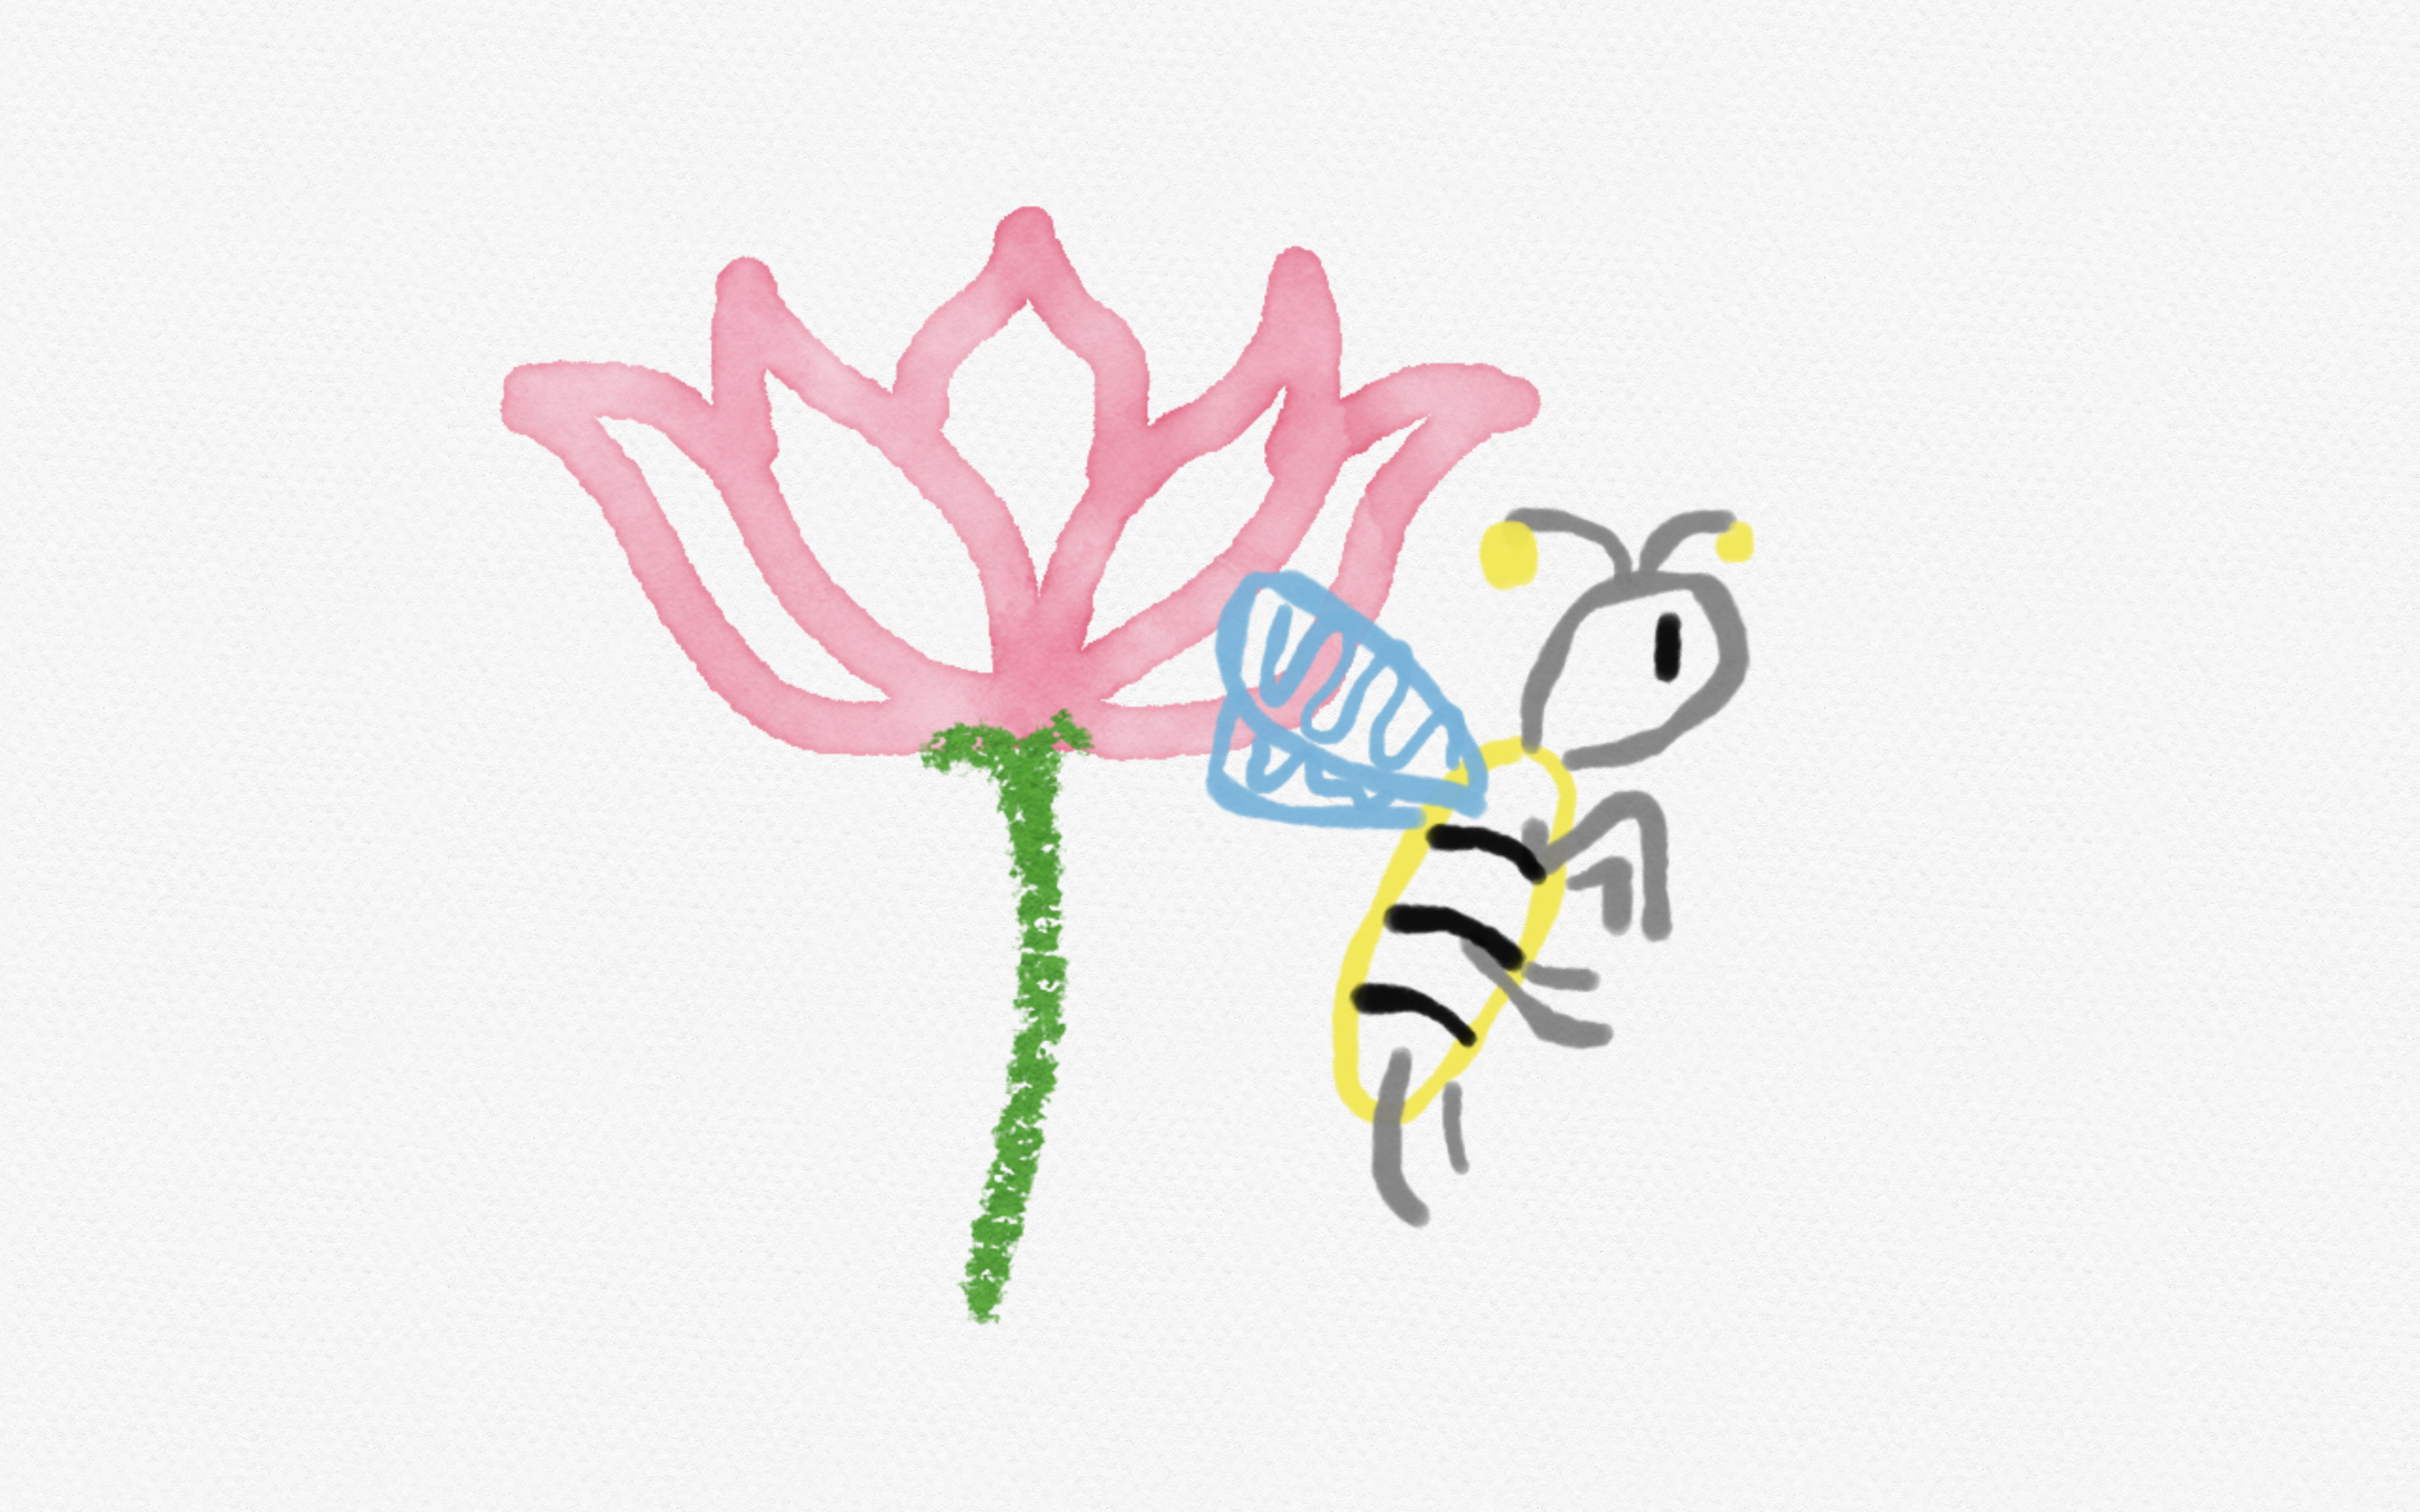
\includegraphics[width = 30em]{Logo}
    \end{figure}
    \newpage
    \tableofcontents
    \newpage

%----------------------------------------------------------------------Kapitel 1--------------------------------------------------------------------------------------------

    \section{Einleitung}
    \newpage
%----------------------------------------------------------------------Kapitel 2--------------------------------------------------------------------------------------------

    \section{Beschreibung der Milensteine}
    \newpage
%----------------------------------------------------------------------Kapitel 3--------------------------------------------------------------------------------------------
    \section{PERT-Diagram}
    \newpage

%----------------------------------------------------------------------Kapitel 4--------------------------------------------------------------------------------------------
    \newpage
    \section{Spezialgebiet}
    \newpage

%----------------------------------------------------------------------Kapitel 5--------------------------------------------------------------------------------------------
    \section{Whiteboxtest}
    \newpage


\end{document}
